\section{ХОД РАБОТЫ}

\subsection{Формулировка задачи}

Рассчитать функции математического ожидания, дисперсии и ковариационной функции
случайного процесса $ \zeta(t) $. Вид составляющих случайного процесса
и распределения их параметров:
$ \zeta(t)= \xi(t) + \psi(t) $,
$ \xi(t) = b $,
$ f_b (\overline{x}) = N(a_b, \sigma^2_b) $,
$ \psi(t) = A \cdot cos(\omega_1 t + \varphi) $,
$ \varphi \in U(-a,a)$.

Параметры $ \lambda = (b, c, d), \varphi, \omega $ предполагаются случайными величинами,
независимыми в совокупности. В символьных расчетах параметры $ b, c, d,
\varphi, \omega $ рассматривать как символьные переменные.

В одно графическое окно вывести десять реализаций случайного процесса $ \zeta(t) $
и функции математического ожидания и дисперсии, моделируя случайные значения
параметров $ b, c, d, \varphi, \omega $.

В отдельное графическое окно вывести график ковариационной функции
случайного процесса $ \zeta(t) $ при выбранных значениях неслучайных параметров.


\subsection{Теоретические сведения}

Математическое ожидание $ a_{\zeta} (t) $, дисперсия $ d_{\zeta} (t) $,
ковариационная функция $ R_{\zeta} (t_1, t_2) $ случайного процесса $ \zeta(t) $
при условии, что $ \zeta(t) = \xi(t) + \psi(t) $ и случайные процессы $ \xi(t) $
и $ \psi(t) $ определены своими конечномерными плотностями вероятностей, рассчитываются
следующим образом:
\begin{align*}
  a_{\xi}(t) &= \int\limits_{-\infty}^{+\infty}  \xi(t, z) f_{\lambda}(z) dz, \\ 
  D_{\xi}(t) &= \int\limits_{-\infty}^{+\infty} (\xi(t, z) - a_{\xi}(t))^2 f_{\lambda}(z) dz, \\
  R_{\xi}(t_1, t_2) &= \int\limits_{-\infty}^{+\infty} \int\limits_{-\infty}^{+\infty} (\xi(t_1, z) - a_{\xi}(t_1)) (\xi(t_2, z) - a_{\xi}(t_2)) f_{\lambda}(z) dz. \\
\end{align*}


\pagebreak
\subsection{Ход работы}

Для выполнения лабораторной работы воспользуемся языком программирования
Python и несколькими библиотеками этого языка:
для выполнения символьных вычислений математического ожидания, дисперсии и
ковариационной функции случайного процесса $ \zeta(t) $ воспользуемся библиотекой
sympy, для подстановки численных значений вместо параметров и отображения функций
на графиках будем использывать библиотеки numpy и matplotlib соответственно.

Исходный код разработанной программы представлен в приложении~А.


В одно графическое окно выведем десять реализаций случайного процесса $ \zeta(t) $,
функцию математического ожидания и дисперсии. В качестве параметров будем использывать
следующие величины: $ A = 2 $, $ w_1 = 1 $, $ \varphi \in (-a; a) $, где $ a = \frac{\pi}{2} $,
$ t \in (0, 10) $ с шагом $ 0{,}2 $ с. Полученные графики приведены на рисунке~\ref{pic:values}.
\begin{figure}[h]
  \centering
  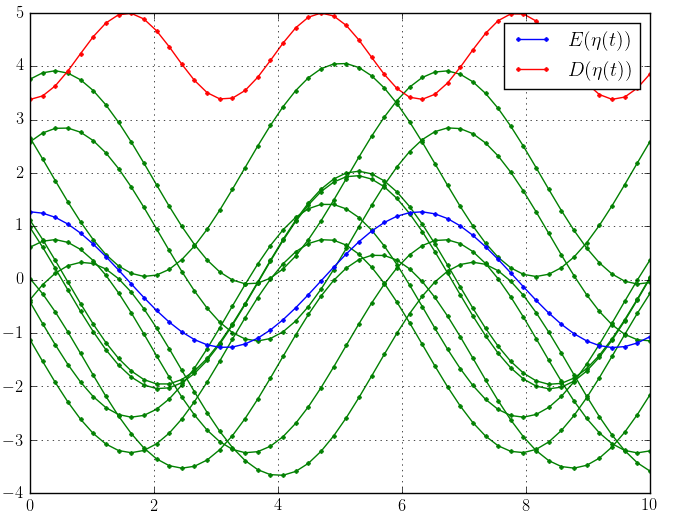
\includegraphics[width=150mm, height=92mm]{pic/values}
  \caption{Графики десяти реализаций, математического ожидания и дисперсии случайного процесса $ \zeta(t) $}
  \label{pic:values} 
\end{figure}

\pagebreak

График ковариационной функции случайного процесса $ \zeta(t) $ приведен на рисунке~\ref{pic:correlation}.
\begin{figure}[h]
  \centering
  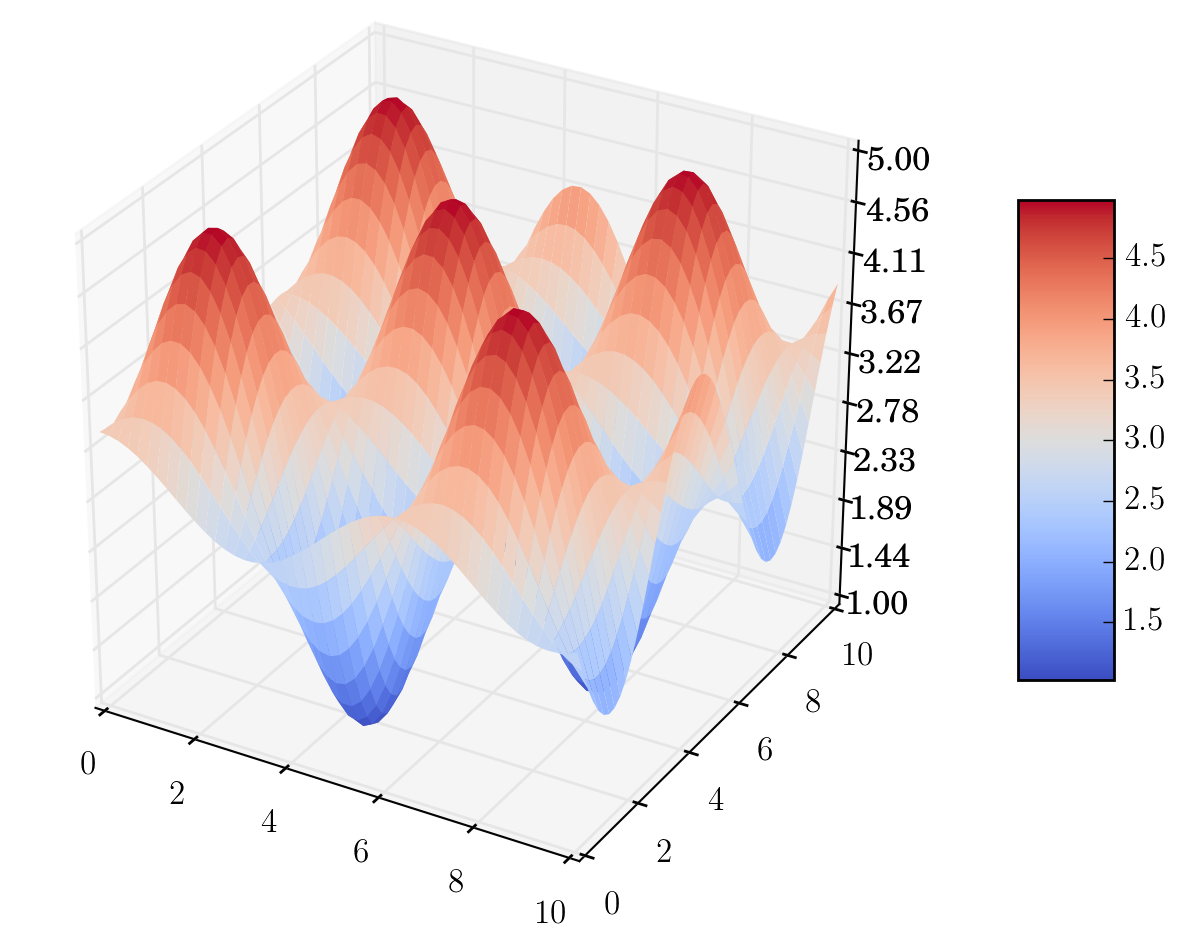
\includegraphics[width=150mm, height=92mm]{pic/correlation}
  \caption{График ковариационной функции случайного процесса $ \zeta(t) $}
  \label{pic:correlation} 
\end{figure}
 
\newpage
